\section{Testbed}
\label{sec:evaluation-testbed}



Our evaluation is based on 3 main experiments. 
The first two are single file download evaluations performed in controlled testbeds in Germany and in the US. 
The third is a real-world website download evaluation performed in Germany. 
In this section we describe the testbeds in more detail. 

All experiments are conducted on a Linux client with $2$ network interfaces. 

The download completion time is the major performance metric. 
It is defined as the duration between the first SYN packet from the client and the last data packet from the server. 
Those values can be retrieved by parsing the client \term{tcpdump}~\cite{URL-TCPDUMP} trace files of each download run. 

\strong{German testbed} 
The real-world measurement and one single file download evaluation are conducted in a testbed in a German university campus. 
The client has one \ethernet~and \wifi~network interface. 
Both interfaces are connected to different networks. 
The university campus has a very large data throughput and latency. 
Consequently, in order to evaluate \mhttp~in a more common environment, we throttle the \ethernet~and \wifi~interface to 15Mbps and 10Mbps respectively, for both, the real-world and controlled testbed evaluation. 

We use 2 Debian machines with \term{Apache2}~\cite{URL-APACHE} servers hosting equal copies of the same files. 
%One server is located on the university campus and the other in a German city named Karlsruhe. 
The Apache servers have resource caching enabled, meaning the files are served from memory and do not require relatively expensive disk IO on the servers. 

\begin{figure*}[!htb]
        \begin{minipage}[t]{0.5\linewidth}
		\begin{center}
                \subfigure[Scenario 1 conducted in German testbed.]{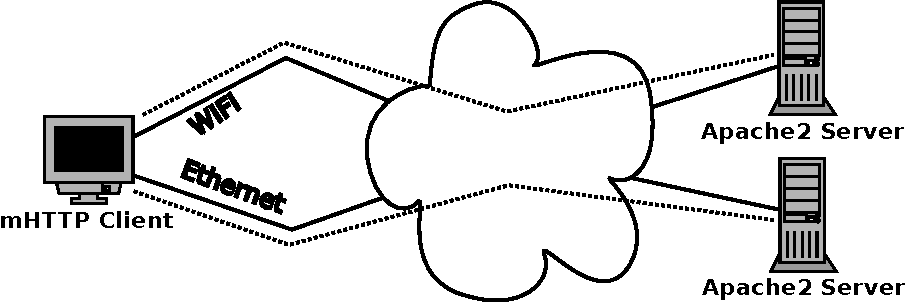
\includegraphics[width=\linewidth]{Figures/evaluation-scenario-1.pdf}}
        \end{center}
        \end{minipage}
~
        \begin{minipage}[t]{0.5\linewidth}
        \begin{center}
                \subfigure[Scenario 2 conducted in US testbed.]{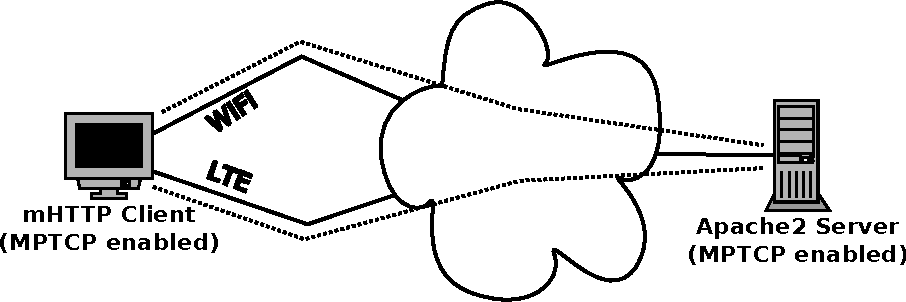
\includegraphics[width=\linewidth]{Figures/evaluation-scenario-2.pdf}}
        \end{center}
        \end{minipage}
        \caption{\label{fig:evaluation-scenarios} Performance evaluation scenario in German testbed (a) and US testbed (b).}
  \vspace*{-0.3cm}
\end{figure*}

For the single file evaluation, inside the German testbed we conduct multi-source tests, meaning both servers are used to concurrently establish connections and download the content, as depicted in~\fref{fig:evaluation-scenarios} (a). 

\strong{US testbed}
In addition to the testbed in Germany, we use an MPTCP enabled testbed in the US \footnote{thanks to Prof. Don Towsley and Dr. Yung-Chih Chen} to get some additional performance data on \mhttp. 
The US testbed is used to compare MPTCP with \mhttp~(with \algslice~scheduling enabled). 
The testbed uses a client with one \wifi~and one \lte~network interface. 
Note, that the MPTCP experiments in this testbed are conducted by our collaborators in the US. 

MPTCP is a single source approach. 
Hence, in order to have a fair comparison, we also use a single server with \mhttp~as depicted in~\fref{fig:evaluation-scenarios} (b). 
Since \mhttp~can freely choose between single- or multi-source downloads, this is not an issue. 
During the experiment, \mhttp~and MPTCP do not interfere with each other, \ie \mhttp~is disabled when MPTCP is running and vice versa. 
